\documentclass[12pt]{article}

\usepackage{enumitem}
\usepackage[right=20mm, left=20mm]{geometry}
\usepackage{type1cm}
\usepackage{amssymb}
\usepackage[fleqn]{amsmath}
\usepackage{tikz}
\usepackage{multicol}
\usepackage{makecell}
\setlength{\columnsep}{1pt}
\usepackage{pgfplots}
\usepackage{float}
\usepackage{caption}
\usepackage{subcaption}
% \usepackage{subfig}
\usepackage{graphicx}

\usepackage{indentfirst}
\usepackage{lastpage}  
\usepackage{fancyhdr}
\pagestyle{fancy}

\usepackage{pgfgantt}
\usepackage[unicode=true,pdfusetitle,
 bookmarks=true,bookmarksnumbered=false,bookmarksopen=false,
 breaklinks=false,pdfborder={0 0 1},backref=false,colorlinks=false]
 {hyperref}

\makeatletter
\newenvironment{myalign*}{\ifvmode\else\hfil\null\linebreak\fi
  \hspace*{-\leftmargin}\minipage\textwidth
  \setlength{\abovedisplayskip}{0pt}%
  \setlength{\abovedisplayshortskip}{\abovedisplayskip}%
  \start@align\@ne\st@rredtrue\m@ne}%
{\endalign\endminipage\linebreak}

% Paper size
\topmargin -10mm
\textwidth 170mm
% \oddsidemargin -5mm
% \evensidemargin -5mm
\textheight 220mm

% Font setting
\usepackage{xeCJK}
% \setCJKmainfont{Noto Sans TC}
\setCJKmainfont{kaiu.ttf}


\renewcommand{\footnotesize}{\normalsize} 
\renewcommand{\headrulewidth}{0pt}
\renewcommand{\footrulewidth}{0pt}

\lhead{}
\chead{2023年全國大專校院智慧創新暨跨域整合創作企劃書}
\rhead{}

\lfoot{}
\cfoot{}
\rfoot{ 共 \pageref{LastPage} 頁 第  \thepage   頁} 

\makeatletter
\begin{document}
\setlength{\parskip}{-6pt}
% \fontsize{14pt}{18pt}\selectfont
% \author{}
\date{}
\usetikzlibrary{automata, positioning, arrows, shapes, fit}
% \maketitle
\tikzset{every state, accepting/.style={double distance=2pt}}
\tikzstyle{block} = [rectangle, draw, fill=white, 
    text centered, rounded corners, minimum height=2em]
\tikzstyle{container} = [rectangle, draw, dashed, inner sep=2em]
\tikzstyle{line} = [draw, -latex']
\captionsetup[figure]{labelfont={bf},name={圖},labelsep=period}
\setlist[itemize]{itemsep=0pt,parsep=0pt}
\setlength{\parindent}{2em}

\noindent
\textbf{參賽隊名:} 普羅程式 \\
\textbf{作品名稱:} 威力導師 PowerTeacher

\section{競賽主題:數位永續科技組}

\section{創作主題}
\subsection{題目:威力導師 PowerTeacher}

\subsection{實用功能描述}
在台灣,資訊科技領域備受關注,且程式設計已成為學校必修課程。儘管每年有數百萬學生修習程式課程,但基層教育仍面臨著許多問題:以往的教學方式需頻繁切換畫面給學生練習、課堂上教師無法即時得知學生狀況。所以我們建立一個名為 PowerTeacher 的網頁應用,專注於教師導向的程式教學工具,整合直播、實作、測驗、互動與AI輔助,讓所有人都能進行優質的程式教學。\\
\par PowerTeacher 是專為教師設計的教學工具,採網頁應用形式,主要提供三種頁面:\\
\par 學生課堂頁面:學生的課堂頁面有直播區、互動區、功能區(見圖x)。
\begin{itemize}
  \item 直播區:用於顯示章節投影片,會在課中展示與老師相同的投影片畫面,並同步老師的滑鼠軌跡、繪畫等。
  \item 互動區:用於顯示滾動式的講義,講義可以放文字、圖片、課堂習題,並且在課中具有引導功能,會根據老師目前的上課投影片,用黃色框線在講義中顯示其對應的位置。
  \item 功能區:用於控制直播區的內容,在課中能夠切換投影片、一鍵回到老師的直播投影片等。在課後能夠拖動時間軸,回放過去的上課直播。
\end{itemize}

教師課堂頁面:教師的課堂頁面與學生的課堂頁面相同,同樣有直播區、互動區、功能區,但功能有部分差異(見圖x)。

\begin{itemize}
  \item 直播區:用於顯示章節投影片,在課中會將畫面同步到學生的直播區中。
  \item 互動區:用於顯示滾動式講義,並能夠預覽課堂習題的作答統計。
  \item 功能區:用於控制直播功能,能夠開啟與關閉直播,在課中可以切換投影片、切換成畫筆功能等。
\end{itemize}

教師講義編輯頁面:教師的講義編輯頁面,用於編輯互動區講義的內容。我們將整個講義分為各種不同類型的小區塊,透過將不同類型的區塊做拼接,以完成整個講義。分為編輯區與時間軸(見圖x):

\begin{itemize}
  \item 編輯區:在右半部點擊不同類型的講義區塊,如文字、選擇題、程式題,就能夠在左半部編輯其中的內容。
  \item 腳本區:下半部的時間軸,用於擺放不同類型的講義小區塊。時間軸的單位是投影片的頁數,讓投影片能對應到不同的講義區塊,在課中就能根據投影片的頁數在講義上做引導與提示。
\end{itemize}

\subsection{作品與市場相關產品差異}

經過與大學與高中程式教師的實地訪談,我們整理出以下三個時間段的教學流程:

\subsubsection{課前:準備教材}

在教學前,教師會準備課堂所需的講義與投影片。市場上的講義編輯功能通常是基於文件編輯器或投影片的形式,例如 Microsoft Word 、Power Point。然而這些工具的功能較為單一,沒辦法嵌入程式執行區、互動習題等與教學相關的功能。我們的平台提供滾動式講義,搭配程式執行、引導、互動習題等功能,使講義內容與課堂做連結。並使用教師講義編輯頁面,使講義更為直觀、易於操作和修改。

\subsubsection{課中:互動教學}

\begin{itemize}
  \setlength{\parindent}{2em}
  \item 直播功能
    \par 實現直播教學的方式,能大致分為硬體與軟體,硬體上常見的有廣播與管理系統,能夠強制控制學生的畫面。軟體上則有 Zoom、Google Meet 等以視訊為主的會議平台或專為學校開發的遠端控制系統,透過網路分享教師的語音與畫面。這些工具分別有幾項問題:前者是強制控制學生電腦,無法讓學生在課堂中與老師同步實作,也無法用電腦查詢資料、觀看講義等。後者是直播的影音可能有延遲,會導致老師的教學與控制不流暢。我們的特色是讓學生能夠在課堂中,操控投影片回顧上課內容,還能同時觀看補充講義、實作程式碼、回答習題等,讓學生就算在課堂中也能回顧與實作,並以更低延遲的直播投影片取代影像直播,使學習更為流暢。
  \item 引導功能
    \par 如何讓學生在課堂中更有參與感並且理解教學內容。市場上的一般教學軟體或平台通常缺乏對於學生學習的引導功能。我們的平台嘗試解決這個問題,透過互動區的黃色框線,在講義中顯示對應的位置,讓學生能夠清楚知道老師目前講解的內容與講義之間的對應。這樣的引導功能可以讓學生更容易理解並隨著教學進度進行,同時也能在回顧時更加方便。
\end{itemize}

\subsubsection{課後:課程回顧}

在市場上,許多教學平台提供課後回放功能,讓學生能夠在課程結束後回顧老師的教學內容。我們的平台也提供了這樣的功能,讓學生能夠在課後拖動時間軸,回放過去的上課直播,以便進一步學習和復習。不過,我們的特色在於,課後回放不僅僅限於觀看直播畫面,還能夠觀看補充講義、實作程式碼等,並搭配引導功能,讓學生在回顧時更為全面與深入。\\
\par 綜合以上幾點,我們整理了老師上課時可能會用到的工具並做比較:

\begin{table}[htb]      
  \centering
  \begin{tabular}{|c|c|c|c|c|c|}
    \hline
    \thead{功能} & \thead{本系統} & \thead{Google Meet} & \thead{遠端控制系統} & \thead{CodingBar}  & \thead{廣播與管理系統}\\ \hline
    直播延遲 & 低 & 高 & 高 & 高 & 低 \\ \hline
    教學方式\footnotemark[1] & 線上與實體皆可 & 線上 & 實體 & 線上 & 實體 \\ \hline
    電腦控制 &  &  & 遠端控制\footnote[2] &  & 完全控制 \\ \hline
    課後回顧 & \checkmark &  &  & \checkmark &  \\ \hline
    線上練習\footnote[3] & \checkmark &  &  & \checkmark &\\ \hline
    教學功能整合\footnote[4] & \checkmark &  &  & \checkmark &\\ \hline
  \end{tabular}
  \caption{老師上課時可能會用到的工具比較}
\end{table}

本系統在直播延遲、教學方式、課後回顧、線上練習以及教學功能整合方面表現出色,並減少對學生電腦的控制,提供了較佳的教學彈性和互動。

\footnotetext[1]{教學方式:教學方式分為線上與實體教學,線上教學指的是在網路平台上進行的教學活動,通常包括遠距視訊教學、線上課程和互動學習模式。實體教學指的是在實際的物理教室或學習環境中進行的教學活動,教師與學生面對面進行互動和知識傳遞。}
\footnotetext[2]{遠端控制:遠端操作是指教師可以強制操作學生的電腦,或者同時與學生在同一台電腦上進行操作。}
\footnotetext[3]{線上練習:線上練習是指讓學生能夠在線上環境中進行練習、測試和應用所學的知識或技能。這種方式可以包括線上測驗、程式撰寫與評測等。}
\footnotetext[4]{教學功能整合:教學功能整合是指將不同的教學元素、工具和方法結合在一起,可以是教學資源、互動工具、直播平台等。}

\section{創意構想}
\subsection{理論基礎}
在與合作教師的訪談中,我們發現教師在教學上面臨以下四項困難:
\begin{enumerate}[label=(\arabic*)]
  \item 使用過多工具的問題:在一門課程中,教師需要使用多種教學工具,包括建置直播、作業平台、設計教材等,這不僅需要讓老師花費較多的時間準備上課環境,還增加了操作上的負擔。
  \item 直播與控制問題:使用網路傳輸為媒介的直播與管理系統,都會有一定的延遲,並且如果控制學生電腦就無法讓學生與教師同步操作,這使得教師在教學上不流暢。
  \item 學生管理困難:教師難以讓每位學生都專注於課程中。
  \item 缺乏即時學習狀況反饋:教師難以即時得知學生的學習狀況,例如學生是否理解課程內容、是否遇到困難等。這使得教師難以及時調整課程進度和教學方式,以更好地滿足學生的學習需求。
\end{enumerate}
為了解決上述問題,我們提出以下基礎以設計平台:
\begin{enumerate}[label=(\arabic*)]
  \item 具連動與整合的介面設計:
  我們將在教學頁面中整合直播、講義、習題和實作,並加入兩者間的引導連動。
  \item 全新的投影片直播方式:
  我們透過同步投影片與教師的操作來實現直播,並採用其他網路傳輸技術以減少延遲。
  \item 加入實作與反饋的功能,以增進師生間的互動:
  在講義中,我們將嵌入程式題和習題,讓學生有機會在課程中進行實作和回答問題。同時,我們的系統將即時統計學生的作答結果,讓教師能夠即時獲得學生的學習情況。
\end{enumerate}

\subsection{設計創新說明}
為符合教師的教學需求,並且以聯合國永續發展目標 SDGs 4. 優質教育為目標,我們的平台將具備以下特色:
\begin{enumerate}[label=(\arabic*)]
  \item 具連動與整合的介面設計:
  \begin{itemize}
    \item 功能整合:在同一頁面中整合直播、實作、課堂習題、講義等功能,讓各種教學元素密切聯繫。這意味著教師能夠在單一平台上完整呈現課程內容,不再需要在不同工具間切換,從而節省了寶貴的教學時間,並使老師跟學生都能專注在課程中。
    \item 互動式講義設計:使用 Markdown 展示課程講義。透過這種滾動式設計,學生在查看講義時不再受到頁面限制,使他們能夠更流暢地瀏覽內容。同時,搭配「引導功能」,透過淺黃色區塊向學生指引出當前投影片對應到講義的哪些部分。這樣的投影片教學方式有助於學生更容易理解並對應到相關的講義內容。
  \end{itemize}
  \item 全新的投影片直播方式:
  \begin{itemize}
    \item 即時同步的直播投影片:此直播系統不同於往常的影像傳輸,而是記錄教師在投影片上的所有操作。包含換頁、繪畫、游標軌跡和聲音實時同步到學生端的介面上,然後存儲在直播記錄中,方便回顧與學習。
    \item 可隨時切換的投影片:為了滿足每位學生的學習需求,我們讓學生在直播過程中,按照自己的學習節奏,切換到其他簡報,並且隨時可以一鍵返回到直播。
    \item 直播回放:學生可以在課後回放過往的直播記錄,並且能夠隨時切換到其他簡報,方便學生複習。
  \end{itemize}
  \item 加入實作與反饋的功能,以增進師生間的互動:
  \begin{itemize}
    \item 嵌入式的程式練習題:可以將程式練習題嵌入至講義的內容中,讓學生可以直接作答,並即時得知答案是否正確以及錯誤的原因。此外,教師也能從教學頁中得知學生的作答狀況,以便於調整教學內容。
    \item 腳本式編輯功能:將互動式講義的內容拆分成多個積木,讓教師能夠針對每個積木進行單獨編輯與編排順序,從而組成一個完整的講義。
  \end{itemize}
\end{enumerate}

\subsection{特殊功能描述}
\begin{enumerate}[label=(\arabic*)]
  \item 講義的互動引導功能
  在課堂中,教師會使用投影片來輔助教學,但學生在觀看投影片時,往往會因為投影片的內容過於繁雜而無法理解。為了解決這個問題,我們在講義中加入了互動引導功能,讓學生能夠清楚知道老師目前講解的內容與講義之間的對應。這樣的引導功能可以讓學生更容易理解並隨著教學進度進行,同時也能在回顧時更加方便。
  \item 低延遲的直播投影片
  傳統影像傳輸的直播面臨著多種延遲和限制。由於涉及多個數據處理步驟,延遲較高。此外,影像與課程教學之間缺乏連接,學生在課堂中無法即時回顧投影片內容。因此,我們採用了一種新的方法,將投影片取代影像,從而讓教學更流暢且與投影片內容緊密結合。
  我們引入全新的直播方式,利用 WebRTC 和 WebSocket 技術,實現投影片與教師滑鼠軌跡和繪畫等的同步。學生和老師可以自主控制投影片的翻頁,這帶來更流暢的課堂互動體驗。
  \item 腳本式講義編輯功能
  為實現投影片和講義內容的對應關係,我們參考了影片剪輯軟體的設計思路,採用了時間軸的概念。我們將講義分成不同類型的小區塊,並在時間軸上將這些區塊組合成完整的講義內容。這樣的設計使教師能夠針對每個區塊進行單獨編輯,並讓講義能隨著上課的流程安排。
  這些小區塊包括選擇題、程式題,以及教師透過 Markdown 語法設計的圖文區。在編排講義時,教師可以輕鬆地將這些區塊放置到腳本區中。腳本區的時間軸對應著投影片的頁數,因此講義的不同區塊能夠與投影片緊密連接。在課堂中,當老師切換到特定的頁數時,就能自動在講義中引導學生目前的上課內容。
  \item 即時程式碼作答反饋
  由於 PowerTeacher 具備自動判讀程式碼的能力,就能在課中自動批改課堂習題,並統計作答結果,能即時得到學生的反饋。
\end{enumerate}

\section{系統架構}

\subsection{架構說明}

\subsubsection{前端(Vue.js)}
使用者界面將採用Vue.js框架來開發,前端主要包括以下幾個部分:

\begin{enumerate}[label=\textbullet, noitemsep]
  \item 直播界面:提供課程直播及實時跟隨課程進度的功能。
  \item 互動式講義:教師可編輯,學生可同步學習並完成練習題。
  \item 作業區(Online Judge):學生可做題並獲得即時反饋,教師可查看結果及統計。
\end{enumerate}

\subsubsection{後端(Gin)}
後端部分我們將採用Golang的Gin框架來開發,後端主要負責以下功能:

\begin{enumerate}[label=\textbullet, noitemsep]
  \item API 提供:為前端提供RESTful API,如獲取課程列表、課程詳情、新增課程等。
  \item 課程管理:儲存和管理課程及章節資訊,並回應前端的請求。
  \item 互動講義管理:處理講義相關的請求,如顯示講義、新增練習題等。
  \item 題目管理:儲存和管理作業及互動式講義練習題資訊,並與judge系統互動。
\end{enumerate}

\subsubsection{資料庫(PostgreSQL)}
我們選擇使用PostgreSQL作為我們的主要資料庫,資料庫將儲存以下資訊:

\begin{enumerate}[label=\textbullet, noitemsep]
  \item 課程資料:包含課程的基本資訊如課程名稱、課程描述、課程章節等。
  \item 章節資料:包含每個章節的基本資訊如章節名稱、章節內容、互動題目等。
  \item 講義資料:包含講義的基本資訊如講義名稱、內容、相關章節、互動性元素等。
  \item 題目資料:包含練習題和互動題的基本資訊,以及用戶的解答狀態和成績等。
\end{enumerate}

\subsubsection{直播系統(WebRTC + WebSocket)}
在我們的平台中,實時課程直播服務將主要聚焦在傳輸老師的聲音以及與學生的互動功能,主要使用以下兩種技術:

\begin{enumerate}[label=\textbullet, noitemsep]
  \item WebRTC:使用WebRTC技術傳輸老師的聲音,實現網頁間的實時通訊。
  \item WebSocket:使用WebSocket技術傳輸老師的滑鼠動作和教學講義的同步滾動,提供全雙工的通訊通道,實現服務器和客戶端的即時通訊。
\end{enumerate}

\subsubsection{judge系統(Judger0)}
judge系統使用Judger0作為基礎,並提供一個安全的沙盒環境來執行和測試程式碼。它能夠與後端的題目管理互動,使得可以讓學生於前端提交程式碼來解決特定的練習題,教師可以使用此功能來評估學生的程式設計能力和理解程度。\\

\begin{figure}[htb]
  \centering
  \href{https://raw.githubusercontent.com/programingtw/proglearn-plan/main/img/powerteacherarc.png}{
    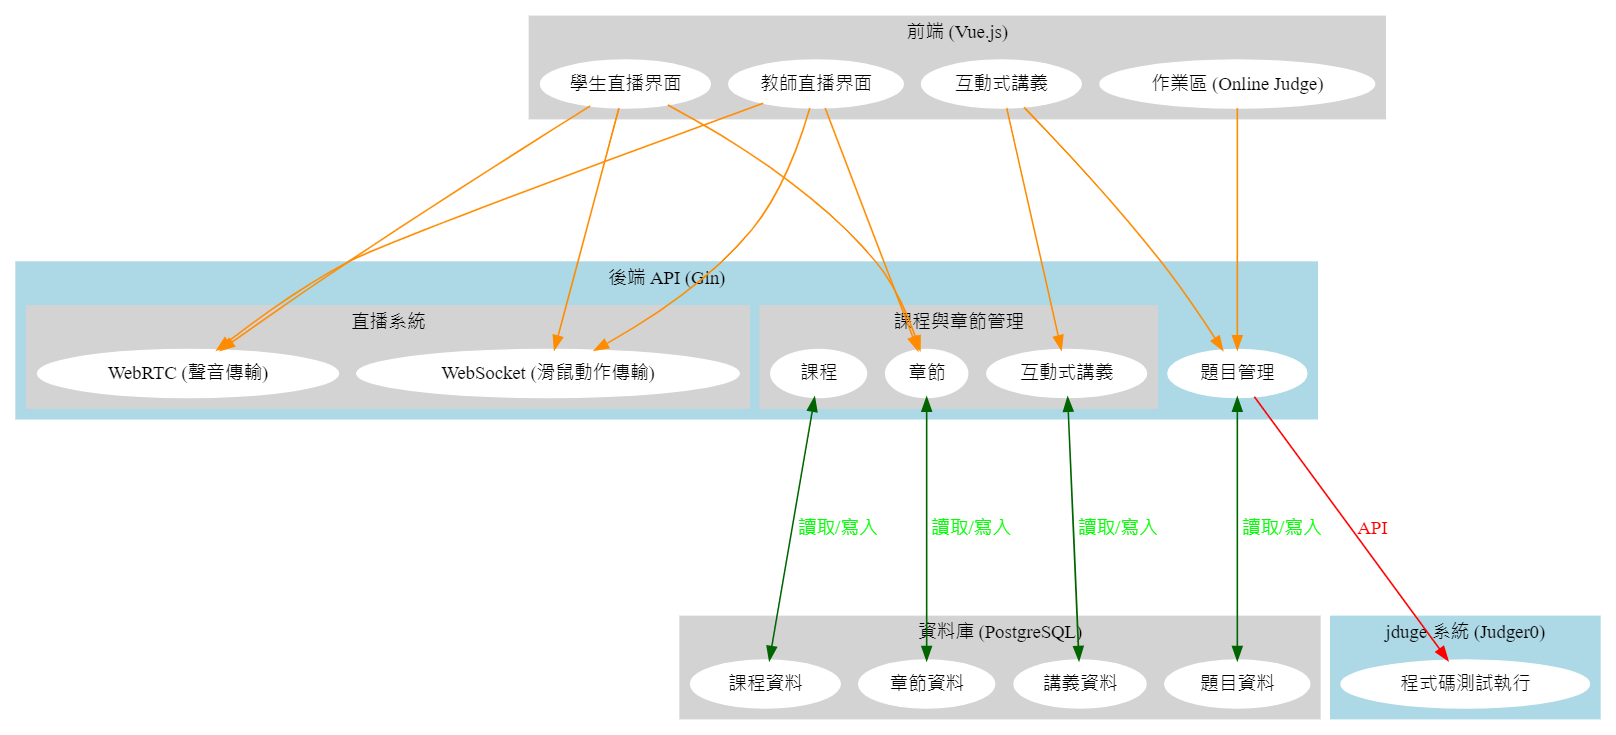
\includegraphics[width=0.5\textwidth]{../img/powerteacherarc.png}
  }
  \caption{系統架構圖}
  \label{arc1}            
\end{figure}

這樣的架構設計是為了使 PowerTeacher 更加模組化和可擴展性,同時能確保每個部分的功能得到最佳實現。例如,前端和後端的分離使得前後端的開發可以並行進行,大大提高了開發效率。選擇 PostgreSQL 是考慮到其高度的可擴展性和穩定性。直播系統的設計則是為了實現更好的即時教學體驗。這套架構能夠滿足 PowerTeacher 的各種需求,並為未來的擴展打下良好的基礎。

\subsection{「人機介面設計」(UI)與「使用者體驗」(UX)設計}

以下使用 Jakob Nielsen 使用者體驗設計優化原則說明:

\subsubsection{Visibility of system status}

\begin{itemize}
  \item 所有課程和章節:使用者在開啟或編輯課程或章節時,系統顯示載入或操作進度。
  \item 投影片上傳:系統在教師上傳教材時顯示上傳進度,並在完成後確認。
  \item 教學頁面:系統在直播進行時顯示播放進度,並在中斷時立即通知使用者。
\end{itemize}

\subsubsection{Match between system and the real world}

\begin{itemize}
  \item 所有課程和章節:課程和章節的結構仿照了真實的教學環境。
  \item 互動式講義:模仿真實的課堂環境,包括教師講解和學生練習。
\end{itemize}

\subsubsection{User control and freedom}

\begin{itemize}
  \item 所有課程和章節:使用者可以自由瀏覽所有參加的課程和已學習的章節,不受限於一定的順序或路徑。
  \item 教學頁面:在觀看回放錄影,使用者都可以隨時暫停、倒退或快進;可自由查看直播、章節概述和互動式講義。
\end{itemize}

\subsubsection{Consistency and standards}

使用 Element Plus UI library 實現了這一原則。

\subsubsection{Error prevention}

\begin{itemize}
  \item 課程與章節管理:系統檢查教師輸入的資訊是否完整和合規,例如確認課程名稱是否已存在,或章節內容是否為空。
  \item 互動式講義:在使用者提交答案前,系統檢查答案格式並提醒使用者確認,避免意外提交。
  \item 投影片上傳:系統驗證上傳檔案的格式和大小,並提供取消上傳的選項,避免非預期的上傳。
\end{itemize}

\subsubsection{Recognition rather than recall}

\begin{itemize}
  \item 課程與章節管理:使用者可以方便地查看已註冊的課程和已學習的章節,並透過搜尋和篩選功能尋找特定課程或章節,降低記憶負荷。
  \item 互動式講義:透過高亮協助學生回憶上次的學習位置,降低尋找學習進度的時間。
  \item 投影片上傳:提供清晰的列表顯示已上傳的投影片或教材,讓教師迅速找到所需的資源,無需記憶與搜尋。
\end{itemize}

\subsubsection{Flexibility and efficiency of use}

\begin{itemize}
  \item 課程與章節管理:快速搜尋和過濾功能,使查找課程更有效率;教師的自由新增和編輯功能,增強了管理課程和章節的靈活性。
  \item 互動式講義:自動儲存學習進度,讓學生能快速回到學習進程;教師可根據課程內容自由編輯講義,提供了教學靈活性。
  \item 投影片上傳:一鍵上傳和管理投影片或教材的功能;支持多種文件格式的上傳,確保了使用的靈活性。
  \item 教學頁面:教師可以自由安排直播時間和內容,提供了教學的靈活性。
\end{itemize}

\subsubsection{Aesthetic and minimalist design}

使用 Element Plus UI library 實現了這一原則。

\subsubsection{Help users recognize, diagnose, and recover from errors}

\begin{itemize}
  \item 所有課程和所有章節:如果某課程或章節不存在,提供明確錯誤訊息(例如「該課程不存在」或「該章節不存在」),並提供回到上一頁或主頁的選項,讓使用者快速恢復。
  \item 互動式講義:提交答案不正確時,提供明確反饋(例如「答案錯誤」或「請再試一次」),並提供解答和解釋,幫助使用者理解錯誤原因及正確答案。
  \item 投影片上傳:如上傳文件格式不支持或文件大小超過限制,提供明確錯誤訊息(例如「不支持的文件格式」或「文件大小超過限制」),並指導如何選擇適合的文件。
  \item 教學頁面:直播中斷或其他問題發生時,提供明確錯誤訊息(例如「直播已中斷,請稍後再試」),並提供可能的解決方法(例如重新加載頁面或檢查網路連接)。
\end{itemize}

\subsubsection{Help and documentation}

\begin{itemize}
  \item 課程與章節管理:課程和章節資訊清晰展示,讓使用者快速了解課程內容和章節進度。提供搜尋和篩選功能,便於找到感興趣的課程或特定章節。
  \item 互動式講義:提供目錄和標籤功能,讓使用者快速找到查看或復習的內容。確保互動題目的正確答案和解釋清晰展示,便於學生自我檢查和學習。
  \item 幫助文件:我們會提供幫助文件,紀錄如何使用系統並包含 Q\&A。
\end{itemize}

\section{計劃管理}

\begin{table}[htb]      
  \centering
  \begin{tabular}{|c|c|c|}
    \hline
    \thead{工作階段} & \thead{工作日數} & \thead{工作內容} \\ \hline
    1 &  &  \\ \hline
  \end{tabular}
  \caption{計劃管理}
\end{table}
\begin{figure}[htb]
  \centering
  \begin{ganttchart}[
    y unit title=0.6cm,
    y unit chart=0.7cm,
    x unit=0.7cm,
    vgrid,hgrid, 
    title height=1,
    progress label text={},
    bar height=0.8,
    bar top shift=0.1,
    ]{1}{8}
    %labels
    \gantttitle{1}{1} 
    \gantttitle{2}{1} 
    \gantttitle{3}{1} 
    \gantttitle{4}{1} 
    \gantttitle{5}{1}
    \gantttitle{6}{1}
    \gantttitle{7}{1}
    \gantttitle{8}{1} \\
    
    %tasks
    \ganttbar{工作階段 1}{1}{2} \\
    \ganttbar{工作階段 2}{3}{4} \\
    \ganttbar{工作階段 3}{5}{6} \\
    \ganttbar{工作階段  4}{7}{8}
    % \ganttbar[progress=0]{工作階段  4}{7}{8}
  
    %relations 
    % \ganttlink{elem0}{elem1} 
  \end{ganttchart}
  \caption{甘特圖}  
\end{figure}

\section{修改舊作參賽說明}
  本專案開發之作品未使用團隊成員曾獲競賽獎勵之作品。
\section{軟體清單}
\begin{itemize}
  \item 作業系統環境:Windows、Linux
  \item 主要開發程式語言:Javascript、Golang
  \item 專案支援語言:中文
  \item 開發環境:
  \begin{itemize}
    \item Visual Studio Code
    \item Node.js
    \item Node Package Manager
    \item Vue 3 Frontend Framework
    \item Gin Backend Framework
    \item Git, Github
  \end{itemize}
  \item 專案成果預定授權條款:本專案開發產品授權條款使用 CC BY-NC 4.0 宣告。
\end{itemize}

\section{權力分配}
依著作權法第 40 條之規定,由參賽學生與指導教授均等共有。

  % \begin{figure}[htb]
  %   \centering
  %   \begin{subfigure}{0.45\linewidth}
  %     \centering
  %     \href{https://raw.githubusercontent.com/programingtw/proglearn-plan/main/img/arc1.jpg}{
  %       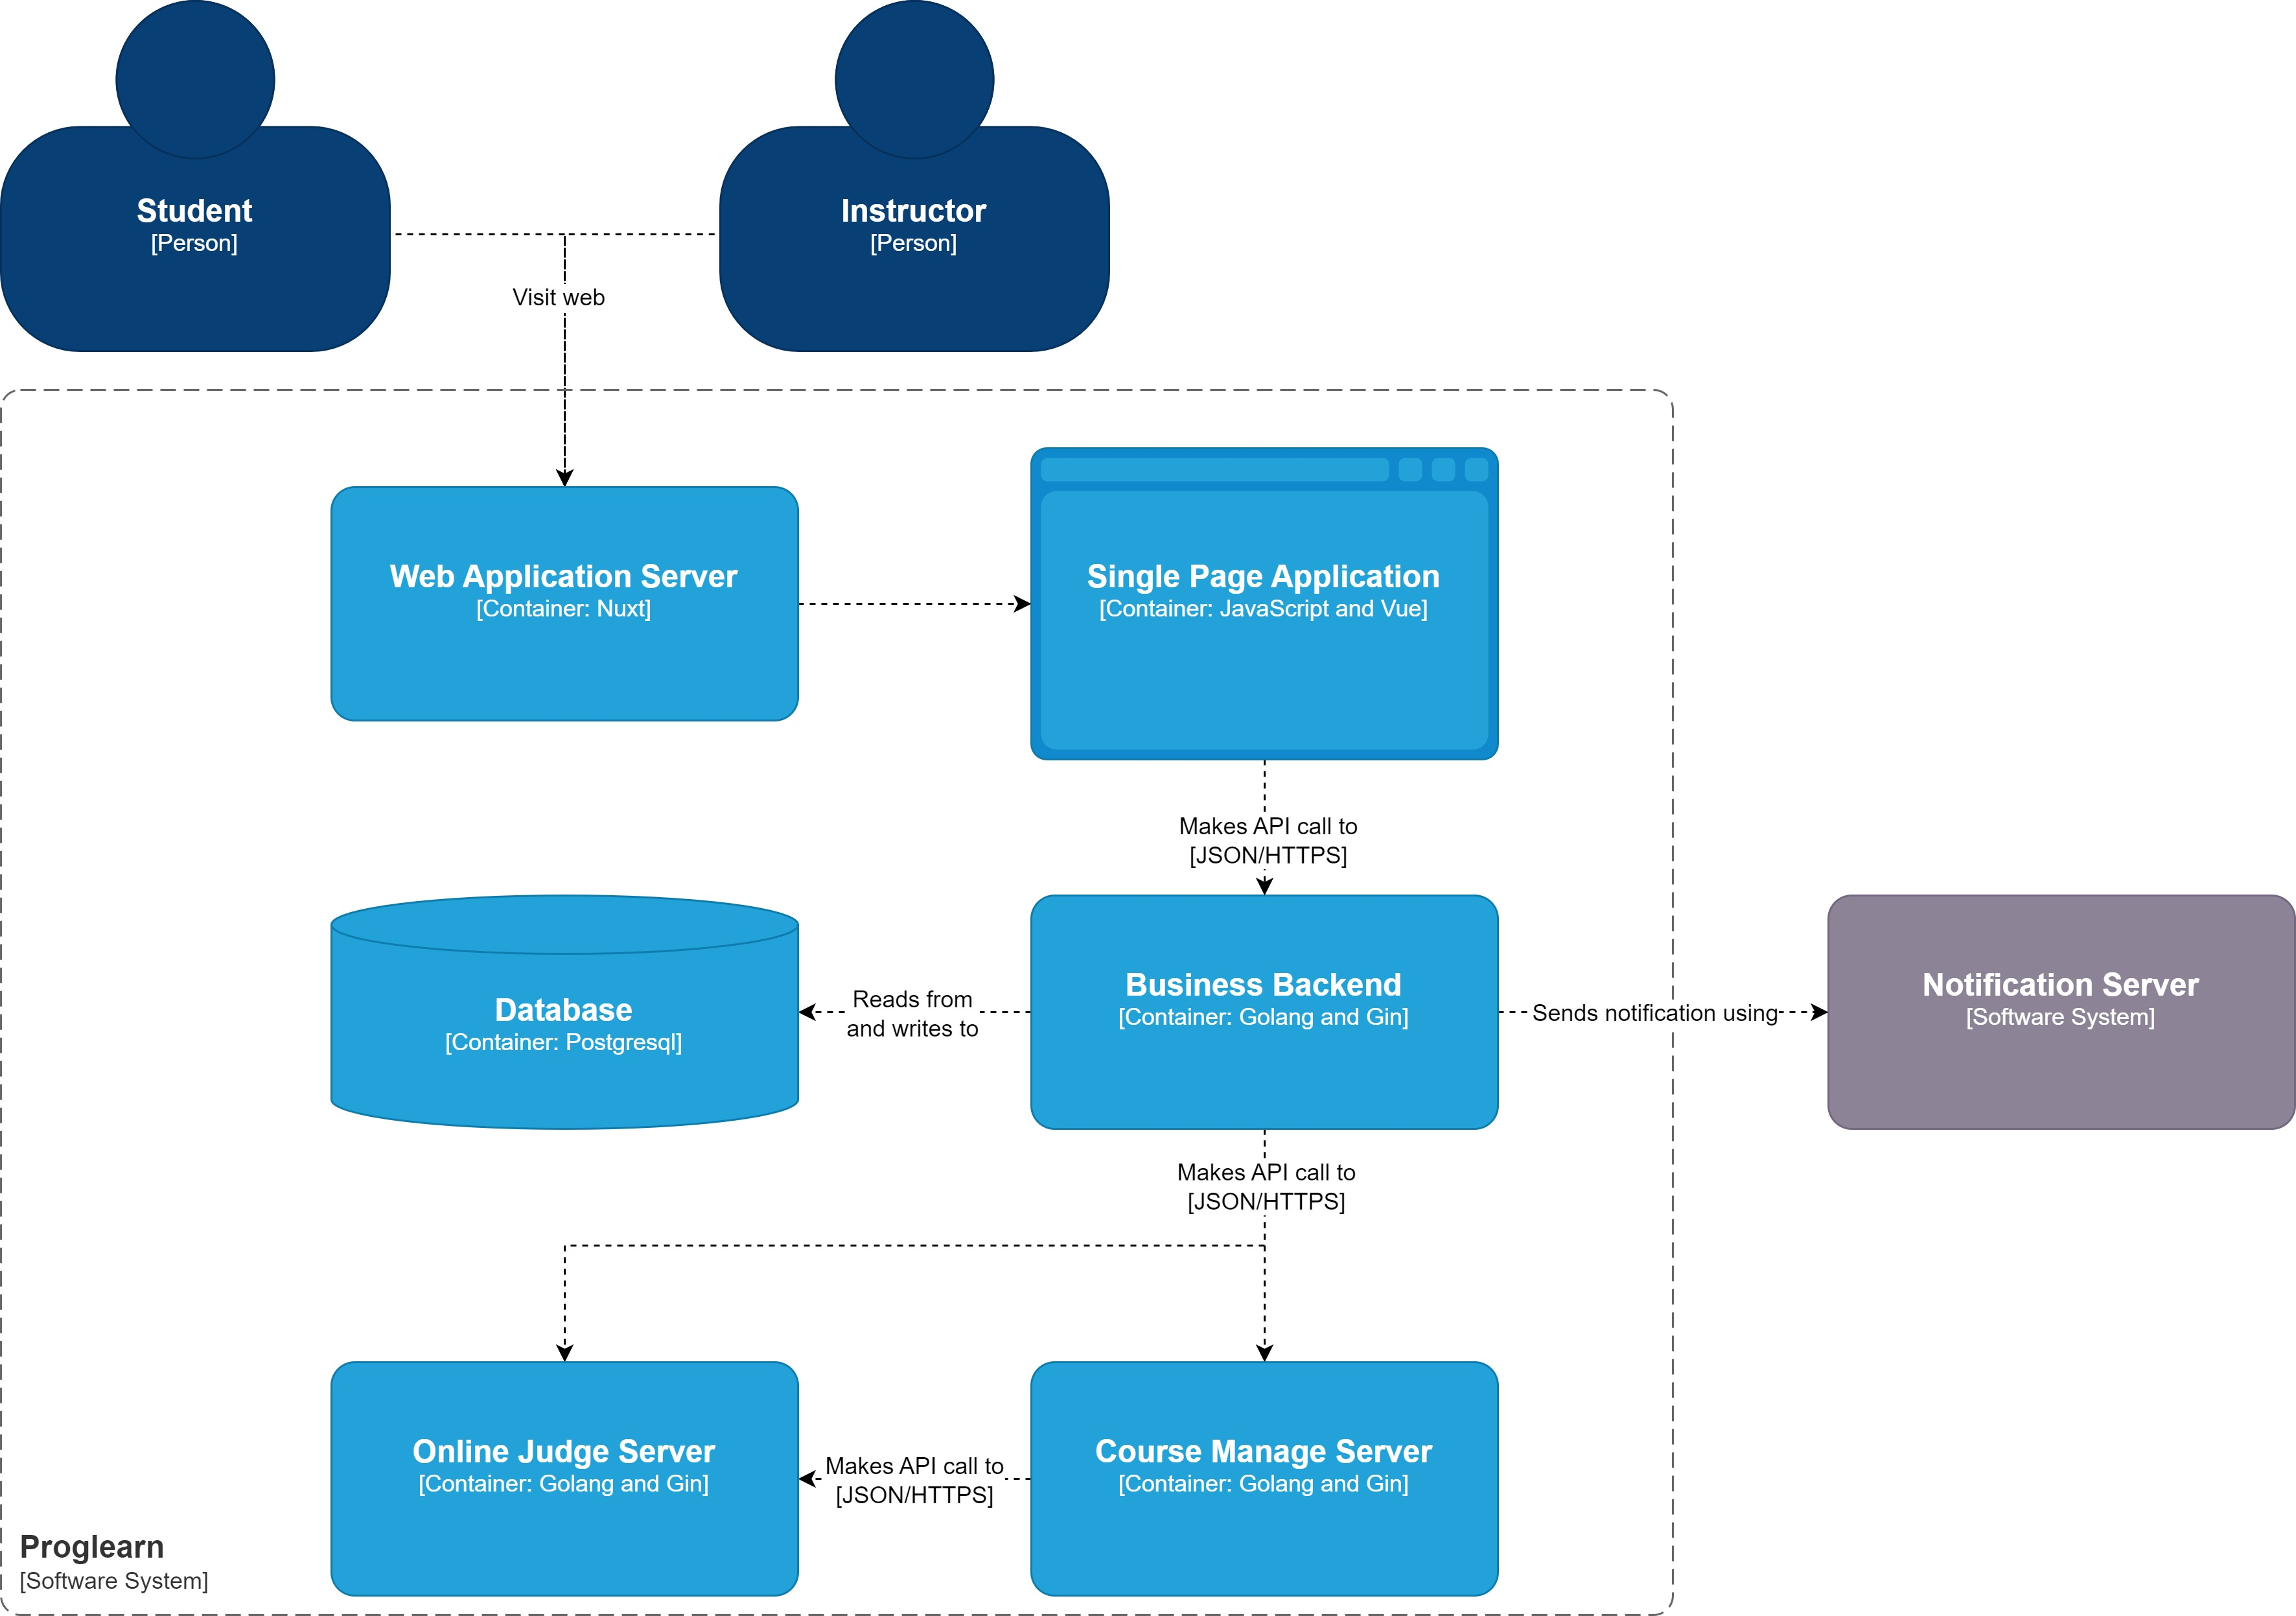
\includegraphics[width=0.65\textwidth]{./img/arc1.jpg}
  %     }
  %     \caption{CAPTION}
  %     \label{arc1}            
  %   \end{subfigure}
  % \end{figure}
\end{document}
